% XeLaTeX can use any Mac OS X font. See the setromanfont command below.
% Input to XeLaTeX is full Unicode, so Unicode characters can be typed directly into the source.

% The next lines tell TeXShop to typeset with xelatex, and to open and save the source with Unicode encoding.

%!TEX TS-program = xelatex
%!TEX encoding = UTF-8 Unicode

\documentclass[11pt]{article}
\usepackage{geometry}                % See geometry.pdf to learn the layout options. There are lots.
\geometry{margin=1.7cm,top=1.0cm,bottom=2.0cm}
\geometry{letterpaper}                   % ... or a4paper or a5paper or ... 
%\geometry{landscape}                % Activate for for rotated page geometry
\usepackage[parfill]{parskip}    % Activate to begin paragraphs with an empty line rather than an indent
\usepackage{graphicx}
\usepackage{amssymb}

\usepackage[compact]{titlesec}
\titlespacing{\section}{0pt}{2ex}{1ex}
\titlespacing{\subsection}{0pt}{1ex}{0ex}
\titlespacing{\subsubsection}{0pt}{0.5ex}{0ex}

% use case command
\usepackage{booktabs}

\newcommand\addrow[2]{#1 &#2\\ }

\newcommand\addheading[2]{#1 &#2\\ \hline}
\newcommand\tabularhead{\begin{tabular}{lp{0.8\linewidth}}
\hline
}

\newcommand\addmulrow[2]{\begin{minipage}[t][][t]{2.5cm}#1\end{minipage}% 
   &\begin{minipage}[t][][t]{0.8\linewidth}
    \begin{enumerate} #2   \end{enumerate}
    \end{minipage}\\ }

\newenvironment{usecase}{\tabularhead}
{\hline\end{tabular}}

% Will Robertson's fontspec.sty can be used to simplify font choices.
% To experiment, open /Applications/Font Book to examine the fonts provided on Mac OS X,
% and change "Hoefler Text" to any of these choices.

\usepackage{fontspec,xltxtra,xunicode}
\defaultfontfeatures{Mapping=tex-text}
\setromanfont[Mapping=tex-text]{Hoefler Text}
\setsansfont[Scale=MatchLowercase,Mapping=tex-text]{Gill Sans}
\setmonofont[Scale=MatchLowercase]{Andale Mono}

\title{Final Project Specification: Miller's Hollow Online}
\author{Team \textbf{Miller's Hollow}
\\Yiyun Yao(yiyuny) \& Jin Wang(jinw2) \& Shangjie Chen(shangjic)}
\date{}                                           % Activate to display a given date or no date

\begin{document}
\maketitle
\section{What is Werewolves of Miller's Hollow?}
\textbf{Werewolves of Miller's Hollow(Werewolves)} is a popular offline discussion game. In the beginning of the game, each player gets one role, which could be a werewolf, citizen or some special roles, such as seer and witch. The game proceeds in alternating night and day rounds.

\textbf{At night}, all players close their eyes and werewolves pick up a victim to kill. After that, special roles can use their skills. For example, a witch can save the victim. \textbf{At daytime}, everyone make a speech to say anything they want, maybe including truth, misdirection and nonsense. After that, players vote to exile one player. The villagers win if all werewolves die. The werewolves win if all villagers die.

For more info, please visit \verb|http://www.playful-pedagogy.org/the-werewolves-of-millers-hollow.html|

\section{What is Miller's Hollow Online?}
Miller's Hollow Online is a website to put the popular game Werewolves online. The original motivation is from ourselves. We all enjoy play Werewolves but sometimes we can't find enough people to play together, or sometimes we don't have enough time and space. Then \textbf{Miller's Hollow Online} is born.

Different from other offline games like cards and chess, the joy of this game is based on its intensive discussion, so we decide to introduce \textbf{realtime video call} in Miller's Hollow Online like Fig. \ref{fig:game}.

In Miller's Hollow Online, apart from playing with friends, users can also play with strangers, which make the game more exciting. There will also be task, tournament and level systems introduced to make this more joyful.

\section{How does it work?}

\subsection{Use Case 1: Building a Room Game}
\begin{usecase}
\addheading{Actor}{Authorized User} 
\addrow{Precondition}{Main page of Miller's Hollow Online is presented to the user with identification}
\addrow{Postcondition}{
A room game with settings and share id is created

The user is added to the room game and selected as the room owner

A room view like Fig. \ref{fig:room} is presented to user
}
\addmulrow{Main path}{
\item User selects Building a Room Game in the main page
\item User selects game type and maximum player number
\item User selects Build button
}
\end{usecase}

\subsection{Use Case 2: Joining a Room Game}
\begin{usecase}
\addheading{Actor}{Authorized User} 
\addrow{Precondition}{Main page of Miller's Hollow Online is presented to the user with identification}
\addrow{Postcondition}{
The user is added to the room game if the players don't reach the maximum size

A room view like Fig. \ref{fig:room} is presented to user
}
\addmulrow{Main path}{
\item User selects Joining a Room Game in the main page
\item User enters shared id of a room game
\item User selects Join button
}
\end{usecase}

\subsection{Use Case 3: Matching Game}
\begin{usecase}
\addheading{Actor}{Authorized User} 
\addrow{Precondition}{Main page of Miller's Hollow Online is presented to the user with identification}
\addrow{Postcondition}{
The user is added to a matching pool in the backend to find a game

The user is added to a matching game

A game view like Fig. \ref{fig:game} is presented to user
}
\addmulrow{Main path}{
\item User selects Joining a Matching Game in the main page
}
\end{usecase}

\begin{figure}
\centering
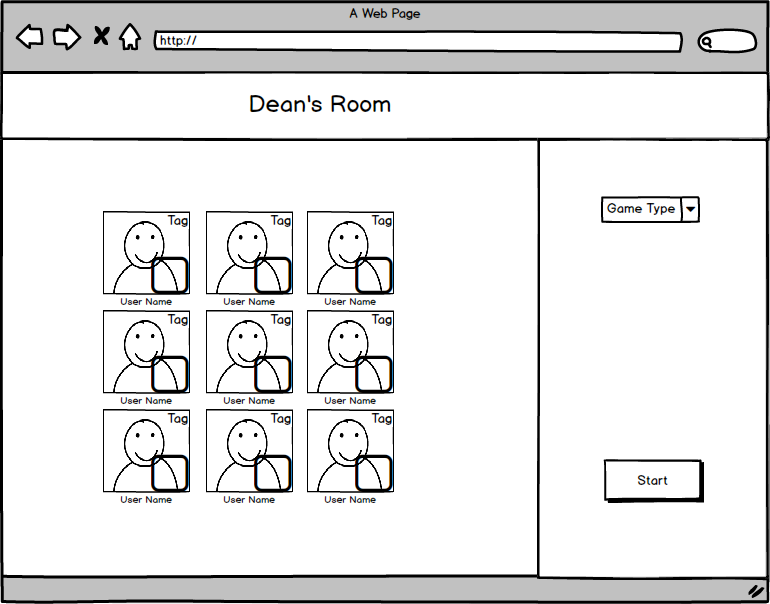
\includegraphics[width=0.7\linewidth, keepaspectratio]{inroom.png}
\caption{Wireframe of Game Room}
\label{fig:room}
\end{figure}

\begin{figure}
\centering
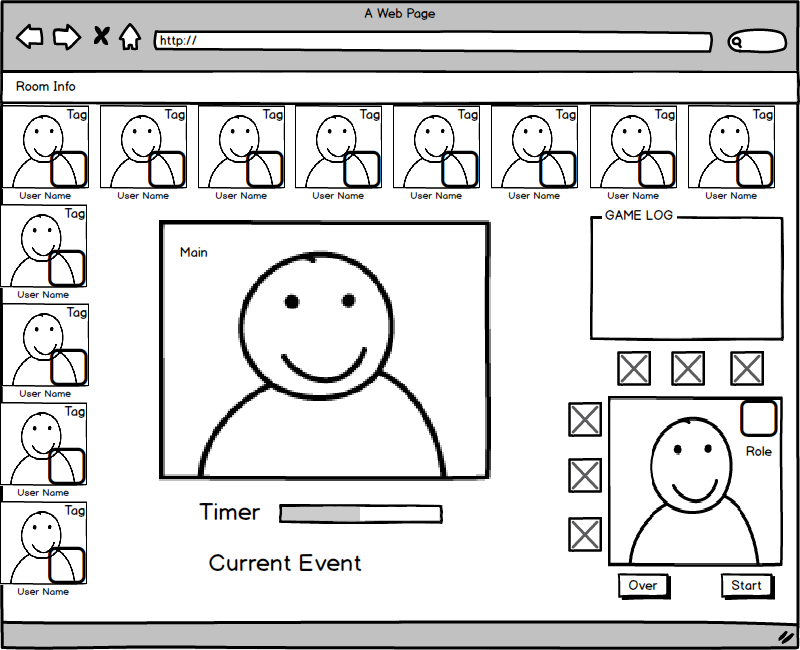
\includegraphics[width=0.7\linewidth, keepaspectratio]{ingame.png}
\caption{Wireframe of Game View}
\label{fig:game}
\end{figure}

\section{What are we going to do?}
\subsection{Technologies \& Division}
\begin{itemize}
\item
Frontend (Jin Wang): AngularJS, phaser
\item
Backend (Shangjie Chen): Django, MySQL
\item
Video transmission (Yiyun Yao): WebRTC
\item
Source Control: git
\item
Continuous Integration: Jenkins
\end{itemize}

\subsection{Requirements}
\subsubsection{Basic}
\begin{enumerate}
\item
Video call available among 9 people, which is the minimum number of Werewolves
\item
A simple sequence of logic with timers to enable players to speak round by round
\item
User authentication and authorization, registration and friend systems
\item
Building room games, joining room games and other utilities in a room, such as getting ready.
\end{enumerate}

\subsubsection{Advanced}
\begin{enumerate}
\item
Full game logic, including changing night and daytime, killing, voting and skills of special roles.
\item
Game log and information alert of game, including current events, voting report and death report.
\item
Interactive user interface in the frontend
\item
Matching game mode, which requires a matching pool in the backend
\end{enumerate}

\subsubsection{Final}
\begin{enumerate}
\item
Communication, task, tournament and level systems
\item
High quality of services
\end{enumerate}
% For many users, the previous commands will be enough.
% If you want to directly input Unicode, add an Input Menu or Keyboard to the menu bar 
% using the International Panel in System Preferences.
% Unicode must be typeset using a font containing the appropriate characters.
% Remove the comment signs below for examples.

% \newfontfamily{\A}{Geeza Pro}
% \newfontfamily{\H}[Scale=0.9]{Lucida Grande}
% \newfontfamily{\J}[Scale=0.85]{Osaka}

% Here are some multilingual Unicode fonts: this is Arabic text: {\A السلام عليكم}, this is Hebrew: {\H שלום}, 
% and here's some Japanese: {\J 今日は}.



\end{document}  